%author : berenice delcroix-oger

\documentclass[border=2pt]{standalone}
\usepackage{tikz}
\usetikzlibrary{positioning, fit, shapes, arrows, calc}

\pgfdeclarelayer{bg}    % declare background layer
\pgfsetlayers{bg,main}  % set the order of the layers (main is the standard layer)

\newcommand{\coula}{0785F2}
\newcommand{\coulb}{F29F05}
\newcommand{\coulc}{F21313}
\newcommand{\could}{E6F21F}



\definecolor{part1}{HTML}{\coula}
\definecolor{part2}{HTML}{\coulb}
\definecolor{part3}{HTML}{\coulc}
\definecolor{part4}{HTML}{\could}

\begin{document}
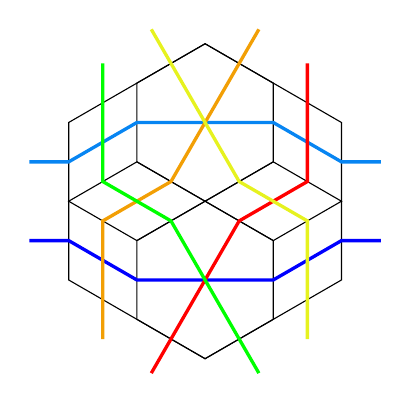
\begin{tikzpicture}
\coordinate (A) at (30:2);
\coordinate (B) at (90:2);
\coordinate (C) at (150:2);
\coordinate (D) at (-150:2);
\coordinate (E) at (-90:2);
\coordinate (F) at (-30:2);
\coordinate (G) at (0,0);
\coordinate (AB) at ($0.5*(A)+0.5*(B)$);
\coordinate (BC) at ($0.5*(B)+0.5*(C)$);
\coordinate (DE) at ($0.5*(E)+0.5*(D)$);
\coordinate (EF) at ($0.5*(E)+0.5*(F)$);
\coordinate (AF) at ($0.5*(A)+0.5*(F)$);
\coordinate (CD) at ($0.5*(D)+0.5*(C)$);
\coordinate (xa) at ($(AB)+(E)$);
\coordinate (xb) at ($(BC)+(E)$);
\coordinate (xc) at ($(DE)+(B)$);
\coordinate (xd) at ($(EF)+(B)$);
\draw (A)--(B)--(C)--(D)--(E)--(F)--cycle;
\draw (AB)--(B)--(BC)--(xc)--(G)--(xd)--cycle;
\draw (G)--(xb)--(DE)--(E)--(EF)--(xa)--cycle;
\draw (AF)--(xd)--(G)--(xa)--cycle;
\draw (CD)--(xc)--(G)--(xb)--cycle;
\draw[part1, very thick]  ($0.5*(A)+0.5*(AF)+0.5*(1,0)$)--($0.5*(A)+0.5*(AF)$)--($0.5*(AB)+0.5*(xd)$)--(90:1)--($0.5*(BC)+0.5*(xc)$)--($0.5*(C)+0.5*(CD)$)--($0.5*(C)+0.5*(CD)+0.5*(-1,0)$);
\draw[blue, very thick]  ($0.5*(F)+0.5*(AF)+0.5*(1,0)$)--($0.5*(F)+0.5*(AF)$)--($0.5*(EF)+0.5*(xa)$)--(-90:1)--($0.5*(DE)+0.5*(xb)$)--($0.5*(D)+0.5*(CD)$)--($0.5*(D)+0.5*(CD)+0.5*(-1,0)$);
\draw[part2, very thick]   ($0.5*(AB)+0.5*(B)+0.5*(60:1)$)--($0.5*(AB)+0.5*(B)$)--(90:1)--($0.5*(G)+0.5*(xc)$)--($0.5*(xb)+0.5*(CD)$)--($0.5*(D)+0.5*(DE)$)--($0.5*(D)+0.5*(DE)+0.5*(0,-1)$);
\draw[red, very thick]  ($0.5*(DE)+0.5*(E)+0.5*(-120:1)$)--($0.5*(DE)+0.5*(E)$)--(-90:1)--($0.5*(G)+0.5*(xa)$)--($0.5*(xd)+0.5*(AF)$)--($0.5*(A)+0.5*(AB)$)--($0.5*(A)+0.5*(AB)+0.5*(0,1)$);
\draw[green, very thick]  ($0.5*(EF)+0.5*(E)+0.5*(-60:1)$)--($0.5*(EF)+0.5*(E)$)--(-90:1)--($0.5*(G)+0.5*(xb)$)--($0.5*(xc)+0.5*(CD)$)--($0.5*(C)+0.5*(BC)$)--($0.5*(C)+0.5*(BC)+0.5*(0,1)$);
\draw[part4, very thick]  ($0.5*(BC)+0.5*(B)+0.5*(120:1)$)--($0.5*(BC)+0.5*(B)$)--(90:1)--($0.5*(G)+0.5*(xd)$)--($0.5*(xa)+0.5*(AF)$)--($0.5*(F)+0.5*(EF)$)--($0.5*(F)+0.5*(EF)+0.5*(0,-1)$);


\end{tikzpicture}

\end{document}
